\documentclass{ip-lab}

\usetikzlibrary{arrows.meta}

\lablevel{n1}
\labnumber{Laboratorio 2}
\labtitle{Funciones}

\makeheader

\begin{document}

\maketitle

\begin{sectionbox}{Preparación}
    Cree un nuevo archivo en Spyder denominado \texttt{n1-l2.py}.
\end{sectionbox}

\begin{sectionbox}{Actividad 1: Área del rombo}
Considere un rectángulo de base $b$ y altura $h$ con un rombo inscrito. Los vértices del rombo tocan los puntos medios de cada lado del rectángulo.

\begin{center}
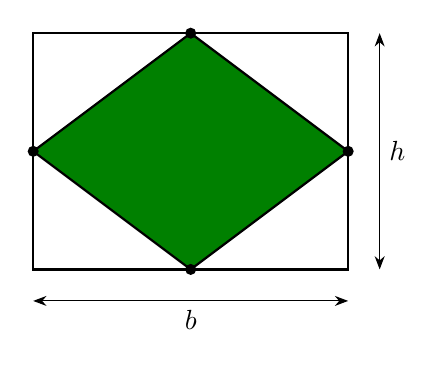
\begin{tikzpicture}[scale=1.0]
    % Shaded rhombus
    \fill[green!50!black] (2,0) -- (4,1.5) -- (2,3) -- (0,1.5) -- cycle;
    
    % Rectangle outline
    \draw[thick] (0,0) rectangle (4,3);
    
    % Rhombus outline
    \draw[thick] (2,0) -- (4,1.5) -- (2,3) -- (0,1.5) -- cycle;
    
    % Midpoint marks
    \fill (2,0) circle (2pt);
    \fill (4,1.5) circle (2pt);
    \fill (2,3) circle (2pt);
    \fill (0,1.5) circle (2pt);
    
    % Labels
    \draw[{Stealth}-{Stealth}] (0,-0.4) -- (4,-0.4) node[midway, below] {$b$};
    \draw[{Stealth}-{Stealth}] (4.4,0) -- (4.4,3) node[midway, right] {$h$};
\end{tikzpicture}
\end{center}

Defina una función llamada \texttt{calcular\_area\_rombo} que reciba como parámetros la base y la altura del rectángulo, y retorne el área del rombo.

\textbf{Consejo:} El rombo se puede pensar como dos triángulos.
\end{sectionbox}

\begin{sectionbox}{Actividad 2: Área de una esquina}
Defina una función llamada \texttt{calcular\_area\_esquina} que reciba como parámetros la base y la altura del rectángulo, y retorne el área de una de las esquinas triangulares que se forman entre el rectángulo y el rombo.

\begin{center}
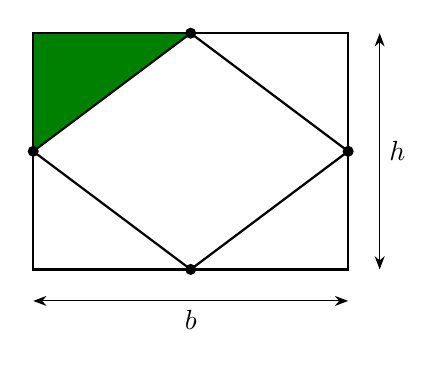
\begin{tikzpicture}[scale=1.0]
    % Only shade top-left triangle
    \fill[green!50!black] (0,1.5) -- (0,3) -- (2,3) -- cycle;
    
    % Rectangle outline
    \draw[thick] (0,0) rectangle (4,3);
    
    % Rhombus outline
    \draw[thick] (2,0) -- (4,1.5) -- (2,3) -- (0,1.5) -- cycle;
    
    % Midpoint marks
    \fill (2,0) circle (2pt);
    \fill (4,1.5) circle (2pt);
    \fill (2,3) circle (2pt);
    \fill (0,1.5) circle (2pt);
    
    % Labels
    \draw[{Stealth}-{Stealth}] (0,-0.4) -- (4,-0.4) node[midway, below] {$b$};
    \draw[{Stealth}-{Stealth}] (4.4,0) -- (4.4,3) node[midway, right] {$h$};
\end{tikzpicture}
\end{center}

\pagebreak

\textbf{Consejo:} Puede reutilizar la función \texttt{calcular\_area\_rombo} de la Actividad 1.

\textbf{Prueba:} Invoque la función \texttt{calcular\_area\_esquina} para un rectángulo de base 8 y altura 6. Muestre el resultado en pantalla usando \texttt{print}. Debería obtener 6.
\end{sectionbox}


\begin{sectionbox}{Actividad 3: Círculo alrededor del rombo}
Ahora considere un círculo centrado en el mismo punto que el rombo, cuyo diámetro es igual a la base $b$ del rectángulo. La región sombreada corresponde al área del círculo que no está cubierta por el rombo.

\begin{center}
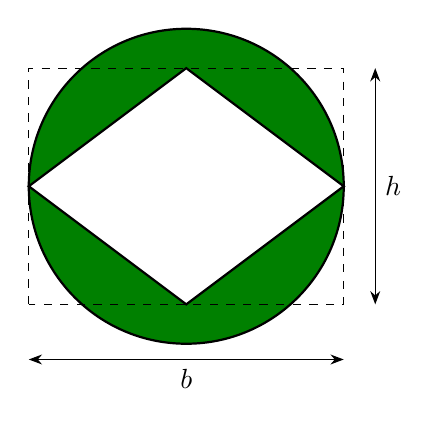
\begin{tikzpicture}[scale=1.0]
    % Shade circle minus rhombus
    \fill[green!50!black] (2,1.5) circle (2);
    \fill[white] (2,0) -- (4,1.5) -- (2,3) -- (0,1.5) -- cycle;
    
    % Rectangle outline (dashed for reference)
    \draw[dashed] (0,0) rectangle (4,3);
    
    % Circle outline
    \draw[thick] (2,1.5) circle (2);
    
    % Rhombus outline
    \draw[thick] (2,0) -- (4,1.5) -- (2,3) -- (0,1.5) -- cycle;
    
    % Labels
    \draw[{Stealth}-{Stealth}] (0,-0.7) -- (4,-0.7) node[midway, below] {$b$};
    \draw[{Stealth}-{Stealth}] (4.4,0) -- (4.4,3) node[midway, right] {$h$};
\end{tikzpicture}
\end{center}

Defina una función llamada \texttt{calcular\_area\_circulo\_sin\_rombo} que reciba como parámetros la base y la altura del rectángulo, y retorne el área sombreada.

\textbf{Consejos:} Puede reutilizar la función \texttt{calcular\_area\_rombo}. Aproxime $\pi$ como \texttt{3.14159}.

\textbf{Prueba:} Invoque la función \texttt{calcular\_area\_circulo\_sin\_rombo} para un rectángulo de base 8 y altura 6. Muestre el resultado en pantalla usando \texttt{print}. Debería obtener aproximadamente 26.3.
\end{sectionbox}

\begin{sectionbox}{Entrega}
Cree un archivo comprimido .zip con el archivo \texttt{n1-l2.py}. Entregue el archivo comprimido a través de Bloque Neón en el laboratorio del Nivel 1 designado como ``L2: Funciones''.
\end{sectionbox}

\end{document}
